\section{Resource Management}
\label{sec:resmgmt}

\subsection{Overview}

At a high level, we designate the \emph{Resource Management} (RM)
thrust as concerning the configuration, scheduling, and
tracking of resources, jobs and users in the \ngrm\ system. The
RM  thrust is a key component of \ngrm\ because it embodies the
user interface to a site's resources and offers the capabilities
for users to submit jobs and thus do useful work with those
resources. Therefore, it is paramount that the RM components of
\ngrm\ not only be generalized, flexible, and extensible, but
also \emph{powerful} and \emph{user-friendly}.

In this section, we will discuss the
components of \ngrm\ that provide our resource managemnt
interface and functionality. With these components, we
aim to fulfil the  goals described above and in
Section~\ref{sect:projorg}. We will start by describing our plan
for a powerful, extensible domain-specific language for use in
describing resources and requests for those resources. We will
continue by outlining the design of a set of global databases that
will be used by our RM software for configuration and historical
data. Next, we will describe the architecture and functionality
of a \emph{job} within \ngrm's unified job model, and how jobs
will interact between parents and children within the resource
management domain. Finally, we will discuss a flexible interface
for job scheduling within the \ngrm\ job, and some details about
job scheduling implementations in the new system.

\subsection{Resource Description Language}

In any resource management system there must be a method by
which the configuration of resources are communicated to the
system. Typically this functionality is achieved via some form
of static configuration, that is via a text file or database
that is created manually or with the help of some kind of
tool. In kind, users need to describe the resource \emph{constraints}
for their jobs in some form -- typically via a combination
of command line options, features requests, and or using
some sort of resource specification language such as the
Globus RSL~\cite{GlobusRSL}.

For \ngrm\ we propose a single resource configuration and
specification language simply termed the resource description
language (RDL).  The RDL shall be a Domain
Specific Language (DSL) that will be used to describe the
hierarchical configuration, topology, and other data about
resources in the system. The language will be structured, extensible,
human-readable, and hierarchical, while being capable of
representing resources and their relationships in a generic and
flexible fashion. It is expected that this language will serve not
only as the base \emph{configuration language} of \ngrm, but that
this language will be the de-facto communication substrate for
gathering resource information such as topology, current resource
state, categorization, as well as constraint specification in
resource requests.

\subsubsection{Related Work}

Fortunately, there exists a large body of literature in this
field on which we can draw when designing the RDL for \ngrm.
While our pragmatic design may not focus on ontological formalism,
there has been work in this area for describing distributed resources
in a Grid~\cite{Castano:2004, Pernas:2005, Koning:2011:UOR:1998662.1998819}
which show promise for semantic matching algorithms on generic resources.
Van Der Ham et al.\ and others have extended the Resource Data Framework (RDF)
specification from the semantic web to describe networked resources
\cite{vanderHam:2006:URD:1160256.1160260, VanDerHam:2008:DTI:2285568.2285672, vanderHam:2006:SHN:1188455.1188643},
and Koslovski et al.\ have developed the Virtual Resources and
Interconnection Networks Description Language (VXDL)~\cite{Koslovski_Primet_2009} for use in
describing the end resources description and virtual network
topology in on-demand virtual infrastructures.

Several other resource management projects have also explored this
area. Possibly most importantly, the Condor project implements
\emph{Classified Advertisements} (ClassAds) which is a language
for expressing not only resources and their attributes, but
requests for these resources~\cite{ClassAd}. The suitability
of resources for resource requests (jobs) are matched using an
array of multi-dimensional gangmatching approaches. The ClassAd
language is available as a standalone library. Additionally, the
OAR resource manager defines resources in a MySQL database with
a static schema, but it does organize resources hierarchically,
allows generic resource definition, and allows users to request
resources using a resource description language~\cite{Oar}. In
the Legion~\cite{LegionGrid,LegionRM} Resource Manager an
inheritance based model is used for defining resources as ``objects''
that are extensible. Another example is CCS~\cite{Keller98ccsresource},
which implemented the Resource and Service Description (RSD)
language and its predecessor the resource description language (RDL).
The RSD in CCS exports not only a language interface for resources
description, but a graphical user interface and API as well.

As part of the design of our RDL, it is expected that we will do a
more complete survey of existing work in this area such that we can
apply common practice and lessons learned to our own implementation
of a resource description and configuration language.

\subsubsection{Resource Description Language Design}

As mentioned above, as part of \ngrm\ development we hope to
create a domain-specific language that is
easily extended and embedded, is human readable, and has the
power to express our hierarchical resource data, topologies,
and advanced resource constraints. The RDL should additionally
have to ability to contain the topology of resources
(which may be different than the heirarchy of the resources).

While a suitable existing encoding may be discovered during
a full literature search, it is our feeling that a solution
based on a static data description or markup language like
RDF or XML is not going to have the ultimate flexibility and
features that we require in the \ngrm.  For this reason, we
currently propose that the Lua~\cite{LuaBook}
language would be a good fit for our requirements.

Lua is a language that was designed to be embedded in other
languages, so it would be easy to embed parsers for the RDL
in various tools. It is also embarassingly easy to extend the
language using modules or directly in native Lua. Finally,
the core datatype in Lua (in fact the only datatype), is
the Lua \emph{table} (an associative array), which lends
itself nicely to the expression of hierarchical data as
we have noted will be necessary for the RDL in \ngrm. There
are many extant examples of the use of Lua as a Data Description
and Domain Specific Language. See the Programming in Lua (PiL)
Book~\cite{LuaBook} for examples.

\begin{lstlisting}[
 float=*htp,
 frame=shadowbox,
 %rulesepcolor=\color{gray},
 numbers=left,
 numbersep=5pt,
 numberstyle=\tiny\sffamily,
 basicstyle=\scriptsize\tt,
 caption={A na\"{\i}ve example of a Lua table describing an excessively simple resource hierarchy},
 captionpos=b,
 label={lst:luaex1}]
ComputeNode = {
  type = 'host',
  attributes = { hostname = '', ipaddr = '', memory = ''},
  children = {
     { type = 'NUMANode',
       id = '0',
       children = {
          { Type = 'Memory', id = '0', value = 16384 },
          { Type = 'Socket', id = '0',
	    children = {
	      { Type = 'CPU', id = '0', children = {}},
	      { Type = 'CPU', id = '1', children = {}}
	    }
	  },
       },
     },
     { type = 'NUMANode',
       id = '1',
       children = {
          { Type = 'Memory', id = '1', value = 16384 },
          { Type = 'Socket', id = '1',
	    children = {
	      { Type = 'CPU', id = '2', children = {}},
	      { Type = 'CPU', id = '3', children = {}}
	    }
	  },
       },
     },
     { type = 'GPU', id = '0' },
  }
}
\end{lstlisting}


Listing~\ref{lst:luaex1} shows a very simple example of
a Lua table used to describe a hierarchy of resources within
a compute node. Note that the attributes of the node resource
are currently left empty, to possibly be filled in as the
table is copied and appended to the {\tt children} table
of another resource, such as a cluster. Used in this fashion --
as a data store -- a Lua table is very similar to JSON, another
popular data interchange format.

It is not expected that the RDL in \ngrm\ will use the na\"{\i}ve
approach as in Listing~\ref{lst:luaex1}. Because Lua is a full
language instead of just a data interchange format, there will be
many optimizations and syntactic abbreviations we can make to ease
working with and using the \ngrm\ RDL.

For example, we expect to use the \emph{object inheritance} support
in Lua to allow resources definied within the RDL to inherit from
other resources. This should support collaboration and research
by allowing sharing of resource definitions as RDL ``libraries''
or resource definition sets. For example, a base type might be
a {\tt Node} class which implements a set of interfaces that are
common to all types of nodes (such as \emph{has a} hostname, ip
address and so on). Specific types of nodes can inherit from the
base node object and add features (such as specialized devices,
default tags etc).

Additionally, with the power of a full language at their disposal,
system managers and users can develop a range of scripts and
extensions that ease working with data in the RM system. For
example, a sysadmin could write a script to create the definition
of an entire cluster by reading a comma-separated value text file,
or other formatted data.

The risks of using a full language like Lua as the RDL for \ngrm\
are also numerous. Since the RDL will be used for resource
requests and definitions, priviliged code within our RM system
may be compiling and running untrusted code. While Lua has very
good native support for sandboxing~\cite{LuaSandbox}, this is
a notoriously difficult practice to get right, and code using
the RDL may need to be hardened extremely well for any use in a
production environment. Evaluation of user-supplied code should
be done within unprivileged processes as much as possible. Also,
when using a dynamically typed, runtime-compiled language like Lua,
there is an increased risk of runtime exceptions, so extra care
must be taken to handle errors correctly, and it is likely that
a specialized "RDL validation" function must be written.

\subsection{Global, Persistent Data in \ngrm}

In the \emph{Unified Job Model} of \ngrm\ we combine the concept
of a traditional job with the idea of a resource management
\emph{instance} which provides the traditional features of a
resource manager and batch scheduler. However, the top-level
\emph{root job} in such a system will need to be initialized from
somewhere. Additionally, in order to be useful, the RM system will
need some sort of persistent record of jobs that ran on the system,
for how long, and on which resources.

To satisfy these requirements, we introduce the global, persistent
\emph{Resource Inventory} and \emph{Job and User Repositores}. These
facilities operate outside of the \emph{hierarchical job model} in
\ngrm\ and act as a source of ultimate configuration and historical
data about the RM system. Each of these facilities is described
in more detail in the sections below.

\subsubsection{Resource Inventory}

As noted above, the Resource Inventory is a global, persistent
database which acts as the top-level configuration for all
jobs within the \ngrm\ system. The resource inventory itself
will support being initialized, modified, and queried using
the RDL, and thus will be optimized for the storage of hierarchical
resources and their topology.
\ifcomments
\marginpar{\tiny
{\bf how} to store hierarchical data and topology information
together is a subject for further research.}
\fi

To satisfy our generalized resource model we must strive to build
a resource inventory that is itself generalized and flexible.
To this end, we propose that the resource inventory implementation
support arbitrary \emph{tagging} of resources. Resource tagging
is a more general approach than the practice of giving nodes
features or properties as in traditional resource managers. We also
propose that the tagging approach is powerful enough to support RM
features such as marking resources \emph{down} or \emph{drained},
an even \emph{allocated}. Furthermore, it is common practice for
tagging databases to allow users to supply their own tags to data
in the system. Use of this kind of \emph{collaborative tagging}
or folksonomy~\cite{wiki:folksonomy}, could be very useful in
creating a socialized system of resource management.

In order to enable the development tools around the resource
inventory, and to support notification of resource changes and
reconfiguration to jobs in the \ngrm\ system, we propose that
the resource inventory export a \emph{subscribe} interface in
addition to a more traditional API. The subscribe interface will
support filtering so that tools (and jobs) can get notifications
of specific changes (perhaps to a subset of resources, or changes
to a particular tag). For instance, the root job in \ngrm\ will
subscribe to the resource inventory to get updates to resources,
such as resources that are drained or modified.

\subsubsection{User Repository}

Since \ngrm\ is a software system that will be used to provide
\emph{users} with access to compute resources, it will require
some place to store information about those users. For this
purpose, we will require a database of user information alongside
the resource inventory. We call this global, persistent user
data store the \emph{user repository}.

At the very least, the user repository will store minimal
data about users of the current deployment of \ngrm. However,
the implemntation should be flexible enough to allow the storage
of other user-specific information, such as defaults, limits,
roles, accounts, qualities of service, and so on.

\subsubsection{Job Repository}

The \emph{job repository} is the final global and persistent
data store in the \ngrm\ system. This top-level database is a
historical record of all jobs that have completed in the
\ngrm\ system. Along with the obvious data about a job --
the start and end times, the resources assigned to the job,
and the owning users -- the \ngrm\ job repository will also
store a complete provenance record for the job. The provenance
record will (configuration permitting) contain data such as the
job environment, namespace or list of installed packages, fault
stream and other job-specific monitoring data. It may also be
beneficial to store other job information such as input files
and stdin/stdout streams, so the job repository will not be
designed with a rigid schema.

Another challenge in designing a job repository for \ngrm\ is
storing job data from the \emph{hierarchical job model}. Similar
to the resource inventory, the job repository will need to be
optimize to store hierarchical data. The intent of the job
repository is to store \emph{all} job data, down to even the
lightweight job invocations in the leaf jobs of the system,
so there will be a mass of hierarchical data here. Developing
a system that not only efficiently represents that hierarcy,
but allows advanced and intuitive queries for the data should
be a top priority.

\subsection{Job Anatomy}
\label{sect:jobanatomy}

The resource inventory and job and user repositories are
not tied to any one job -- they exist at the global, persistent
level in \ngrm\ and export a common API.  To fulfil the unified
job model, however, each \ngrm\ job must contain all the
same features implemented by these global databases, but local
to the job. For this purpose, we introduce the concept of
an \ngrm\ \emph{instance}, which is the embodiment of all
resource management features at the job level.

The components of an \ngrm\ instance are outlined in
Figure~\ref{fig:rminstance}.  These components largely match the
global, persistent data store described in sections above, but since
jobs in our RM system may be ephemeral, these implemenations are
lightweight and may be started on-demand instead of being always
instantiated. This practice of minimizing the functionalitly
instantiated per instance will not only serve to reduce the cost
of starting and stopping the software for every job, but optimizes
for the \emph{base case} job in \ngrm\ -- a single job running a
single parallel application.

\begin{figure}
\centering
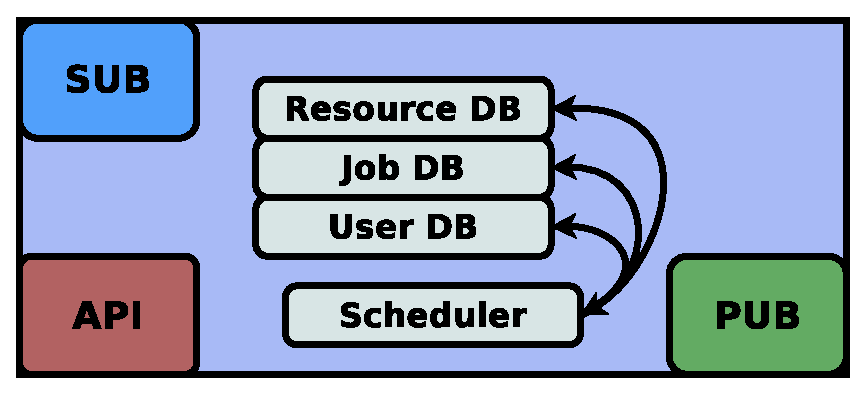
\includegraphics[scale=0.30]{../fig/RM-instance.eps}
\caption{Components of a Resource Manager Instance}
\label{fig:rminstance}
\end{figure}

Within an instance, we give these temporary counterparts to the
global, persistent databases a new name to differentiate them. They
become simply the resource, job, and user databases. Each of
these job-local databases contain only the subset of information
which applies to the current job. For example, the resource DB
will have information only about resources assigned to the job, the
user DB will have only the users allowed to run within the job and
the job owner, and the job database will contain information only
for jobs that have run in the current job or a completed child.

As a whole, the RM instance exports similar API and publish interfaces
as the top level persistent databases. For instance, most interaction
with the instance functionality of a job will be through the well
defined API. However, other functionality may be more adapted to
a PUB/SUB interface, for example a parent job will subscribe
to its children for events of interest, and child jobs may subscribe
to parents for information trickling down from higher levels in the
hierarchy. Interesting changes in this context may include data
about resources in the child (this resource is dead), information about
the child itself (I'm dead), or information about resources from
the parent (this resource is being drained in 20 minutes).
\ifcomments
\marginpar{\tiny
Instance API and pub/sub interface is a topic of future research. }
\fi

Below, we discuss in slightly more detail the resource, user, and
job databases. Detailed descriptions of these components in the
context of the job lifecycles are described in later sections.
We also take this opportunity to touch upon the
scheduler interface within the RM instance. However, a detailed
scheduler discussion is saved for a later section.

\subsubsection{Resource Database}

The resource database within a job is expected to be implemented as
a read-write \emph{cache} of the job's subset of the parental resources.
The resource data for a job must be writable in order to satisfy
the \emph{self-hosting} requirement of \ngrm. An owner of a job
should be able to update tags and configuration of resources within
their job, however, non-privileged user tags and configuration will
be marked as such, and so shall not affect upstream or ancestoral
job or resource configuration.

\subsubsection{User Database}

The user database within a job contains, at a minimum, the job
owner along with an optional list of users that are allowed to
access the job. As described above, the user database may be
as simple as a list of user names, but it is extensible enough
to be used for an array of other user-specific data -- preferences,
roles, limits, and qualities of service are just some examples.

In \ngrm\ we would like to grant users the ability to \emph{invite}
other users to submit jobs to a job for which they are the owner.
A simple example of this functionality would be the root job,
which is owned by user \emph{root} and to which \emph{all} users
are invited. However, other use cases for this functionality
include dedicated application tests (DAT) in which a coordinater
may invite a group of users, or a debug session on a large running
running job where debugging experts may be ``invited'' to run some
diagnostics. To support this functionality, we propose that the job
\emph{owner} should be able to add users to the user database, and
that those users would then be able to submit new job requests to
the instance. Users with \emph{submit} access shall not have access
to runtime functionality of the job, nor the ability to initiate
lightweight jobs. However, it other circumstances it may be useful
to have the ability to expand the list of users that \emph{do}
have such access.  Therefore the user database must support both
\emph{submit} and \emph{runtime} access lists for jobs, though it
may be wise to make these lists optional based on configuration.


\subsubsection{Job Database}
\label{sec:jobdatabase}

The job database serves the same purpose as the global job repository
within an instance, but additionally acts as the data store for pending
and running jobs within the instance. Jobs are submitted to a local
instance via the API. The syntax and validity of job requests are checked
and the job request is passed through a set of plugins that may modify
or reject the job based on site-specific requirements. Valid job
requests are inserted into the job database, at which point a
``job created'' event is generated. Scheduler and other plugins may
then act upon this event.

The job database will also support generating ``job start'' and ``job end''
events.
\ifcomments
\marginpar{\tiny
The exact list of events generated by the job (and other) database
is a topic of future study. It may be useful to research a method
to allow \emph{arbitrary} events from all these datbases. However,
the ``job state change'' events are key, so they are called out
explicitly here.} \fi

\subsubsection{Scheduler Plugin}

Another major component of the RM instance is the job scheduler.
The scheduler is discussed in more detail below, however here we
note that the scheduler implementation is provided by a plugin,
and that the loaded scheduler is configured at the time of job
instantiation. Thus, while it is expected that the root job will
likely have an advanced, complex scheduler plugin loaded, most jobs
running in the RM system will have a default, simplistic scheduler
implementation, or perhaps no scheduling code loaded at all, if
it is unnecessary. It is also important to note a scheduler plugin
(or any other RM instance plugin) is running within the context of a
\ngrm\ job. Therefore, these plugins have access to the full power
of the the distributed job environment for use in parallelizing
work and distributing state for fault tolerance and scalability.

\subsection{Job Physiology}

We have briefly described the RM components in the \ngrm\ above.
In the sections below we expand on this discussions and begin
to describe how processes within a job interact with the containing
job, and how the RM instances within jobs in the \emph{hierarchical model}
interact with eachother.

\subsubsection{The Root Job: \emph{Job 0}}

In our hierarchical job model, every job in \ngrm\ has a parent
and zero or more children jobs. It is obvious, however, that
the root job (or \emph{job 0}), does not have a direct parent.
In this special case, the resource inventory acts as the
indirect parent of job 0. When the root instance is bootstrapped
by the CMB, the root job connects to the global, persistent
\ngrm\ databases and recieves just enough resource, user, and other
configuration data to initialize. The root instance then
\emph{subscribes} to the resource inventory so that it is
notified of important changes.
\ifcomments
\marginpar{\tiny
Again, the list of ``important'' changes is a subject of further
study. However, an administrator could tag a resource `down' in the
resource inventory and job 0 would then be notified immediately through
its subscription. This would trickle down to the appropriate progeny
via the pub/sub channels in each instance}
\fi

Once the root job is initialized, it may become the de facto interface
for users to the system, i.e. the instance within job 0 may
provide the interface for all users of \ngrm\ at a site for
job submission, queries, and other RM-related work. In this
case, jobs are submitted to the root job's API and are
inserted into the job database as described in Section~\ref{sec:jobdatabase},
and the job 0 scheduler will prioritize and schedule these
requests.

In our system, however, this is not the only scenario. The
flexibility of the unified job model allows a site to invoke
sub-jobs of job 0 and reference those jobs as respective interfaces
to subsets of resources within a datacenter.  For instance, to run
in a more traditional mode, a centerwide root job could spawn one
sub-job for each cluster within a datacenter. These cluster-specific
jobs would then act as separate ``resource managers'' for these
clusters, and could therefore have different scheduler plugins
loaded, a different set of users, or other separate policies.
However, even in this case, it is important to note that job 0 still
spans all the resources in the center, so job data is eventually
collected in the top-level job repository, all resources in the
center are configured in a singular resource inventory, and a
centerwide runtime and monitoring environment exists for use by
administrative tools.

\subsubsection{The \ngrm\ Job: \emph{Job $n$}}

As explained in the sections above, a job requests in \ngrm\ are
always submitted to an existing \ngrm\ job via the instance API.
This job request is passed through a set of configurable plugins
which check the validity of, and make any modifications to, the
new job request. If the request is valid, and the requesting user
has submit access to this job, then the job request is inserted
into the job database as described in section~\ref{sec:jobdatabase}
above.

After the scheduler has determined the job should run and
resources have been selected for the job, a new comms session
is spawned, and the CMB intiates the new instance for this
job, which we call job $n$. The instance is initialized using
the universal resource description language  of \ngrm\, which
will describe the set of resources assigned to the job. Once the
new instance is initialized, it will subscribes to its parent
instance (for notification of upstream resource changes, and
other items ``of interest''), and the parent subscribes to the
child instance. Finally any script or interactive session is spawned
within the job, with configuration such that RM utilities and
APIs will utilise the URIs specific to the job $n$ instance.
\ifcomments
\marginpar{\tiny
TODO: Flesh out the details here. Need to describe batch vs interactive
vs ``pure allocation'' jobs.
}
\fi

Upon initialization, ownership of job $n$ is set to the submitting
user, and that user would typically be the only user allowed
access to the runtime environment of the job. However, the list
of users with submit access and runtime access is configurable
and may be set after job invocation or during the job request
itself.

It is also not necessarily the case that the instance invoked by
the job --  that is, the set of daemons and code that provide the
RM instance features in \ngrm\ -- are of the same versions as the
parent job. In fact, part of the design of the self-hosting, unified
job model of \ngrm\ is to allow not only \emph{rolling updates}
of software, but to allow future and experimental versions of the
software to be deployed as an \ngrm\ job. This means that
the version of the software system used within a job may be
user-selectable, or for privileged users a version of the
tool could be loaded directly from a build directory.
\ifcomments
\marginpar{\tiny
A study of the security implications of these features is outstanding.
However, it is expected that \emph{certain} pieces of software would
be deemed safe to allow blanket per-job user replacement rules. (e.g.
the scheduler)
}
\fi

Once job $n$ is running and fully initialized, user processes
have access to a rich and powerful private resource management system
for use in directing  their computational work. Information
about resources can be gathered and stored in the local
resource database, which in turn can direct and optimize
behavior of the in-job scheduler. Chained jobs and workflows
can be inserted into the local job database and child jobs can
be created which in turn use the power of their local RM system
to manage related work. Every sub-job and parallel invocation
is captured in the local job database, along with monitoring
data streams and other job data which can be used in postmortem
analysis and job efficiency studies.

A graphical representation of a typical set of jobs showing
jobs running within jobs and their respective instances is
shown in Figure~\ref{fig:RMComponents}.

\begin{figure}
\centering
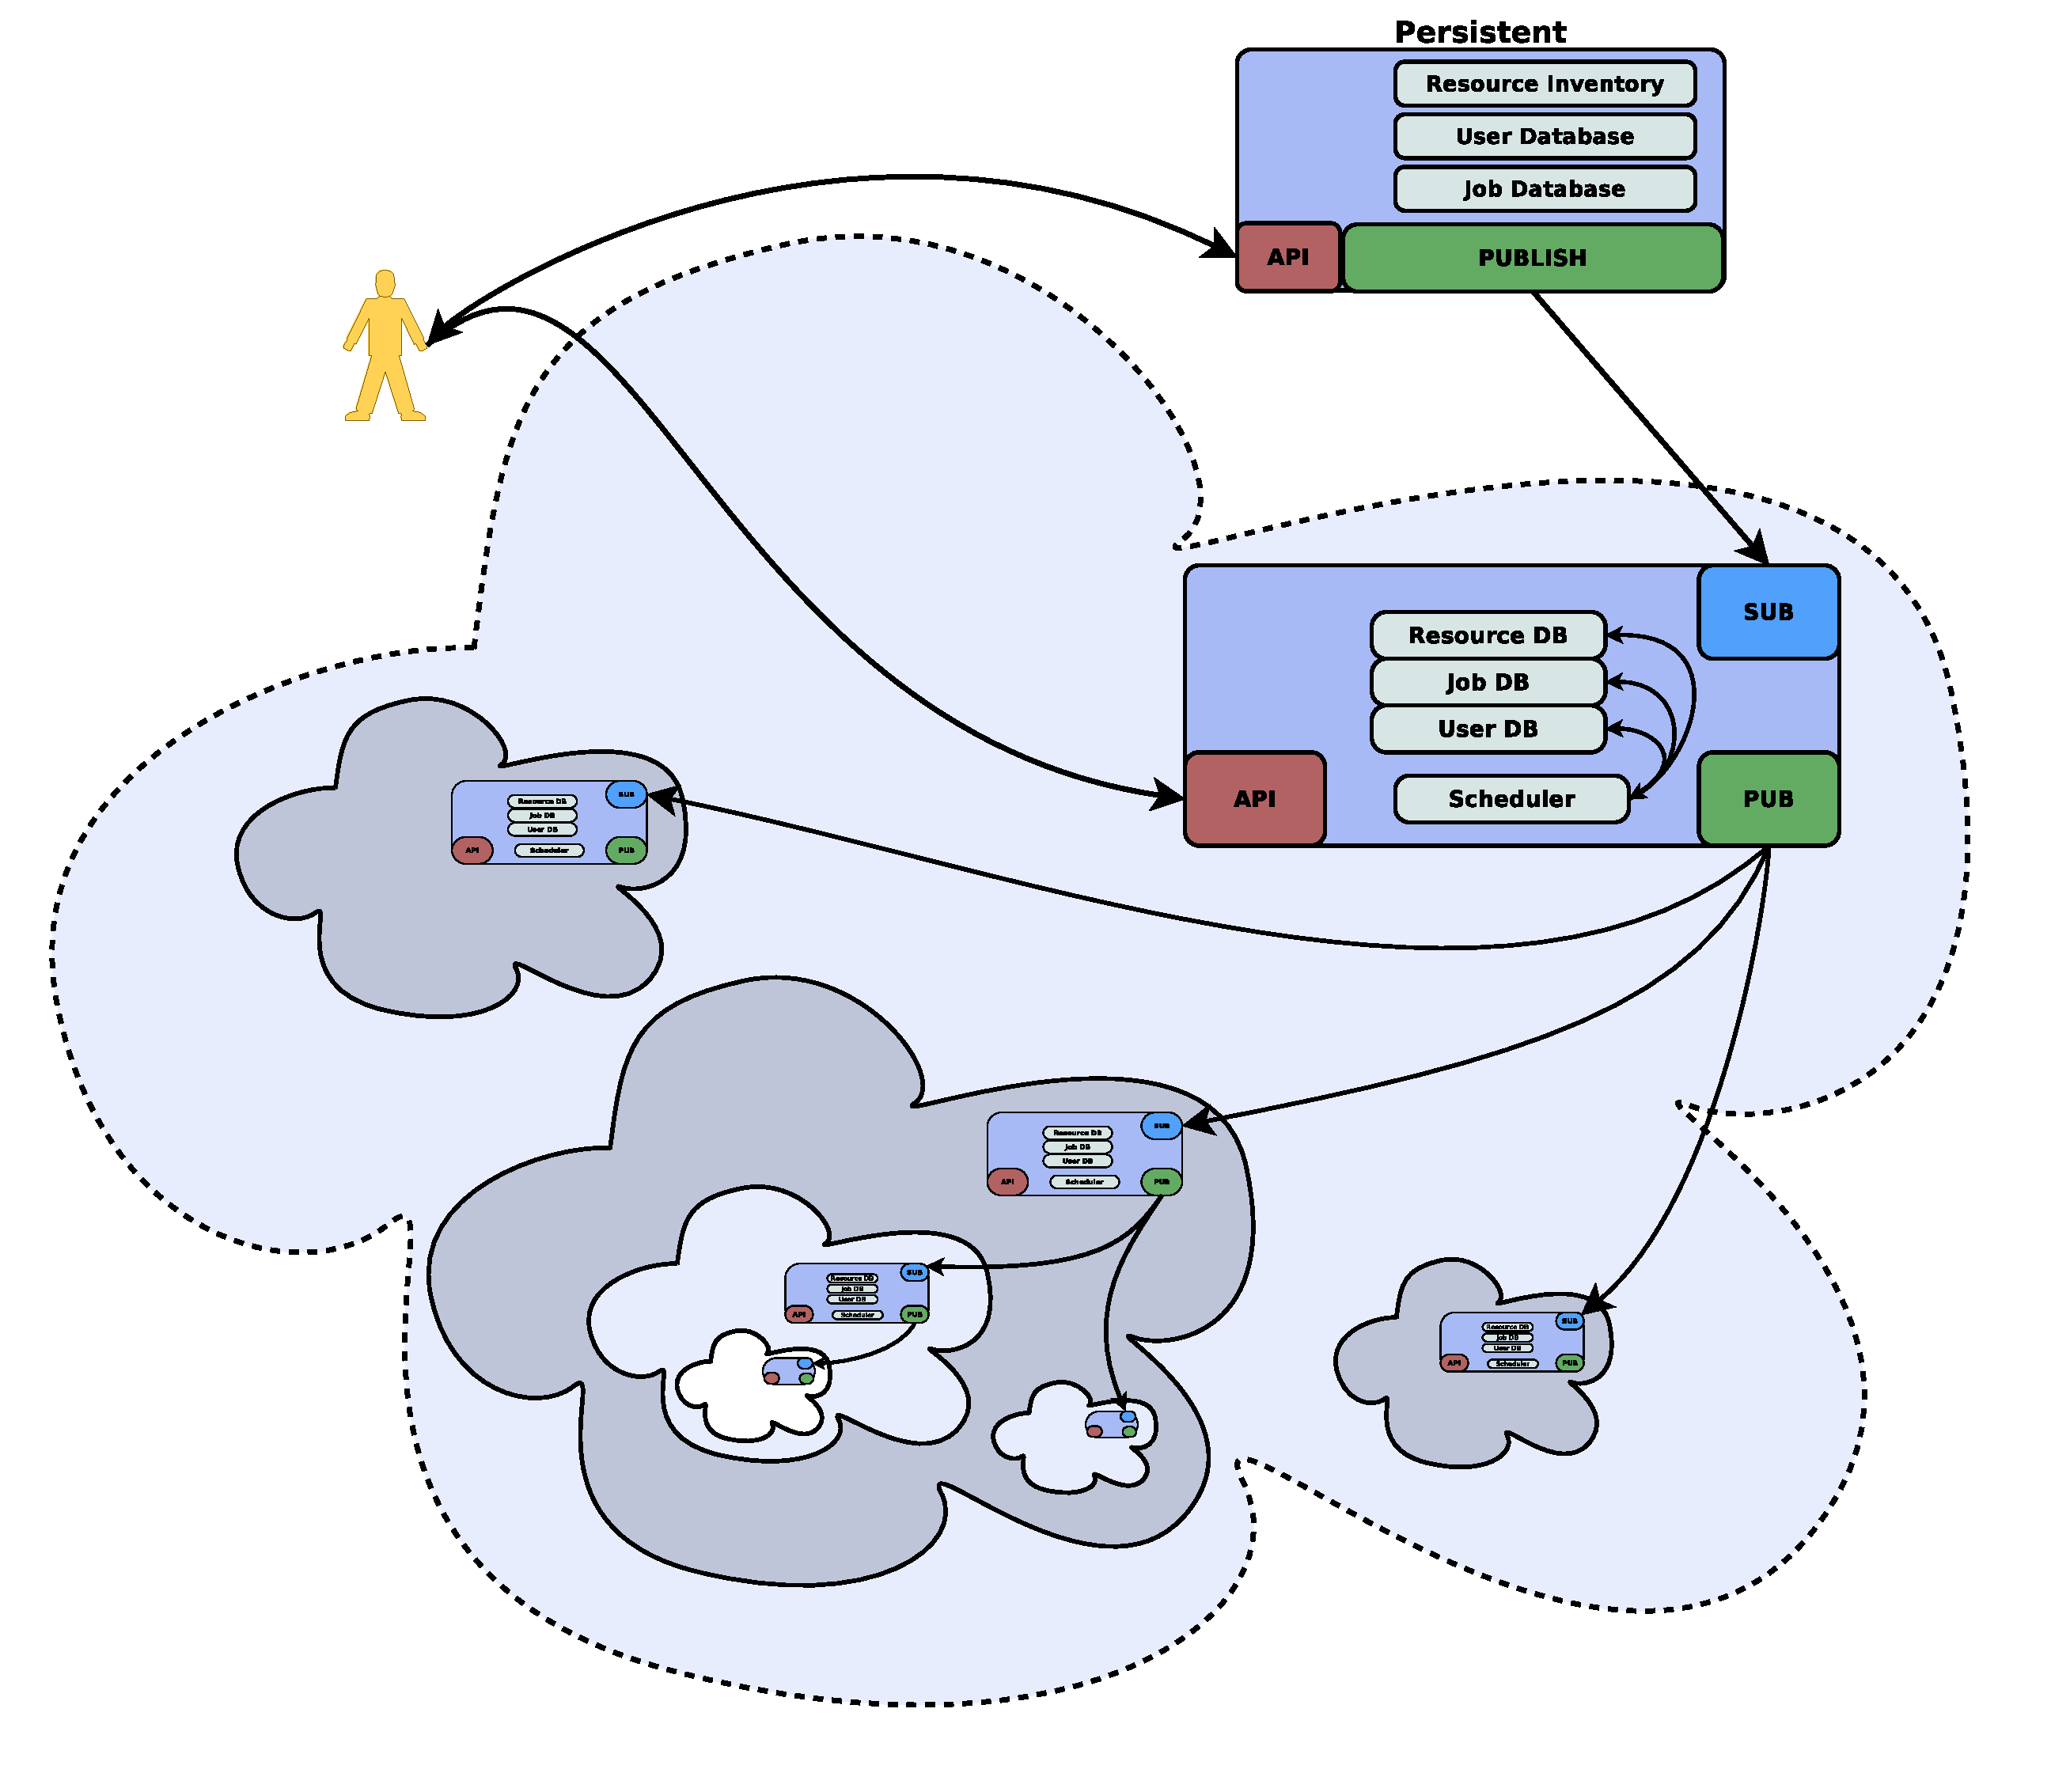
\includegraphics[scale=0.20]{../fig/RM-full.eps}
\caption{Resource Manager High Level View}
\label{fig:RMComponents}
\end{figure}


\subsubsection{Lightweight Jobs}

As described earlier, lightweight jobs (LWJ) are similar to normal
jobs in the \ngrm\ system, but they do not result in a new
instance. Thus, these jobs run within the current instance and
utilize the same scheduler, resources, and other instance specific
data. It is expected that lightweight jobs will be the vessel by
which parallel applications are launched and managed, and this
topic will be explored further in the workload and runtime section.

For the RM instance within the job, all the same steps are taken
when handling a lightweight job vs.\ a normal job.  There may only
be a flag or tag that indicates this job will be \emph{lightweight}
instead of requesting the instantiation of a full job. This approach
is beneficial because it reduces code duplication in handling the
distribution and management of processes local to the runtime of
the current job. Another benefit of treating lightweight jobs
as a special case of regular jobs is that the lightweight job
information will be captured in the job database and preserved,
just as any other full job.

One final note about lightweight jobs is that it will likely be
necessary to allow lightweight jobs instantiated on the system
to overlap. For example, one LWJ might be a parallel MPI application
running across all nodes of a job, and second, overlapping
LWJ would be a parallel debugger session used to attach to one
or more of the processes in the original job. Again, both of
these jobs would be captured in the job database.
\ifcomments
\marginpar{\tiny
TODO: What happens when a LWJ request comes from within a LWJ.
I think it is Dong's assumption that LWJ's have their \emph{own}
hierarchy -- so the current level in the hierarchy would need
to be communicated to the RM instance, and the instance would
need to manage that hierarchy.
}

It is assumed that the lifecycle management of LWJs will be
handled at the level of the runtime environment. It may not
be possible in all cases to determine exactly when a LWJ
is ``complete'', and it may be up to the user code creating
the LWJ, or the runtime subsystem doing so on behalf of
the user, to explicitly notify the RM instance when
a LWJ has completed.

\subsubsection{Job End-of-Life Care}

We will adopt a model from UNIX process management and have the
parent instance "reap" its children. It is here that the job db from
the child can be "pulled" up from the child into the parent job db.
When instance 0 reaps jobs, this job data can be pushed up to its
parent, i.e. the persistent job repo.

\ifcomments
\marginpar{\tiny
TBD -- how to store child job information in the parent such that the
historical lineage of the jobs and sub-jobs within the child are
preserved.  Maybe the reaping should be abstracted down in the comms
layer with callbacks to allow the higher level subsystems to reap
their analogs in children.
}
\fi

In this model, historical job data makes its way up to the top-level
job repository as child jobs complete. Each "running" job instance has
information about its historical job lineage in its local job db, so
this information can also be queried directly from within the context
of a job. (e.g. in a DAT, if you want to only query information about
jobs from the DAT, you can query the DAT job instance. In fact,
information about jobs from the DAT are not populated to the top-level
job repository until the DAT "ends")

We will define how jobs indicate that they are "done" and need to be
reaped. A DAT "job" may need to be killed and reaped at the end of its
time limit. Normal batch jobs are complete when the batch script
running on the control node exits. A direct allocate/launch with WRAP
would be reaped when the processes being launched exit. A job may
be forcibly killed by the user or an administrator, at which point
a depth-first recursive termination is issued.

\ifcomments
\marginpar{\tiny
TBD -- What happens to an active job hierarchy when the top-level job
is killed?  What happens to pending job requests when a job is
terminated?  Killing a job might result in something like:

\begin{enumerate}
\item Freeze local job db (i.e. disallow new job submissions)
\item Terminate and reap children jobs
\item Kill local tasks
\end{enumerate}
Perhaps 2,3 could be swapped or done in parallel.
}
\fi


\subsubsection{Job Fault Tolerance}

While discussing job interactions, it rapidly becomes apparent that
an important feature of the \ngrm\ job will be its tolerance of
faults in the RM instance. If there is data loss within the instance,
then this may affect the data of all completed child jobs, since
hierarchical data such as the job database are generally collected
in the parent after a \emph{reap} operation. While fault tolerant
design is a goal of \ngrm\ design and a topic of further study,
we mention here some initial ideas for job recovery after RM
instance failure.

One possibility is to build the resource, job, and user databases
on top of a distributed data store with replication. The runtime
environment of job will already contain a distribute key-value store,
so it may be possible to build a fault tolerant data store on
top of that. With replication enabled, the failure of a node
on which the RM instance is running would not be fatal because
the data could be reconstructed from replicas.

Another proposal is to replicate data to other instances running
in the system. For example, a job could replicate data to its
children and parent, and a lost instance could then be reconstructed
by the parent by querying missing data from the children. This
method would require a systematic method for determining location
of child jobs without help from the parent, but it is expected
that this challenge is not insurmountable.

Because the impact of losing job instances while running may be
large, in fact larger than in some other RM software systems,
our development should focus on testing this case, and ensuring
that there is no undesired data loss when an RM instance crashes
or its host goes down should be part of a routine test plan.


\subsection{Job Scheduler}

The \ngjs\ is responsible for scheduling computing resources to users'
jobs.  Users submit to the scheduler requests for resources to run
their job.  The scheduler implements management's policy to decide
when and where to allocate the resources for each job.

This section summarizes the requirements for the \ngjs, a rough design
which meets those requirements, and a work breakdown structure for
developing the scheduler component.

\subsubsection{Motivation}

Scheduling batch jobs across a collection of networked computing
resources connected in a grid has been a common paradigm for at least
two decades.  A batch scheduler receives users' job requests, selects
a cluster for each job, then dispatches the job to that cluster's
resource manager to be executed.

The \ngjs\ represents a departure from traditional monolithic ``grid
masters''.  The scheduler functionality will be a service provided by
the \ngrm's job model.  As such, the scheduling activities will be
distributed across the center's resources and provide functionality
not available in any commercial or open source project.

\ngjs's scheduling services will schedule jobs across resources in a
computing center without regard to current cluster boundaries.  A job
will be able to request resources containing a common feature (like
connectivity to the same high speed switch) or fitting within a
limited power envelope.

The \ngjs\ will support plugin modules that provide unique scheduling
behavior and job prioritization.  Each job will have the option to
independently load its own scheduling plugin.  In so doing, the
\ngjs's scheduling capabilities will range from scheduling all
resources in the center to scheduling jobs on dedicated resources
(DATs) to scheduling LWJ's (job steps).

Most importantly, the traditional boundaries between a job scheduler
and the resource manager will be redefined under \ngrm.  Instead of a
resource manager that manages every resource of a cluster, the
resource management services will be instantiated as part of the job
and be restricted to only the resources allocated to the job.

In order to continue to meet the needs of current users, the
\ngjs\ must continue to provide all the services that production
schedulers provide.  Our goal is to surpass our existing schedulers in
the following areas: performance, accuracy, reliability, resiliency,
ease of use, flexibility, security, diagnostics, and need for manual
intervention.

\subsubsection{Requirements}

While a more detailed list of requirements is presented in
\ref{ReqsHiLevFun}, the following provides an overview of the
functionality that the \ngjs\ will be expected to deliver.

\paragraph{Fundamental Requirements}

The following is the most definitive list of basic scheduling
requirements.  The job and resource repositories as well as the job
submission facility are external to the \ngjs.

\begin{itemize}
  \item Prioritize each job
  \item Schedule each job based on its resource requirements
\end{itemize}

\paragraph{Further Scheduler Requirements}

In addition, more elaborate scheduling plugins will be provided to do
the following:

\begin{itemize}
  \item Support complex job dependencies, e.g. as in scientific workflows
  \item Backfill lower priority jobs whenever possible
  \item Facilitate dynamic job growth and reduction
  \item Preempt running jobs to free up resources needed by higher priority jobs
  \item Calculate estimates of when each job will begin
  \item Provide scheduling answers to ``what if'' scenarios
  \item Scheduling different resources to a job over time
\end{itemize}

\paragraph{Policy Enforcement}

\ngrm\ implements the center's policies for providing access to its
computing resources.  The following are responsibilities,
traditionally associated with a batch scheduler, that will be borne by
the larger \ngrm\ system:

\begin{itemize}
  \item Reject job submissions for jobs which cannot or will never run
  \item Remove jobs that exceed time limits
  \item Enforce established limits on users, groups, projects (banks), etc
  \item Honor service level agreements and service quality requests
\end{itemize}

\paragraph{Organization Components}

The \ngjs\ functionality is broken down into the following components.

\textbf{Job Prioritization.}  This the facility for prioritizing jobs
based on potentially multiple factors.  The system shall offer a job
priority plugin framework to allow custom algorithms for determining
job priority.  The priority of each queued job must be continually
recalculated as the queue of jobs and workload factors change.

\textbf{Job Scheduling.} For each job removed from the prioritized
queue, computing resources must be reserved and eventually allocated.
The collection of resources to schedule must be available from the
resource inventory with the state and status of each resource updated
in real-time.  The scheduler must honor multiple resource requests
simultaneously as it seeks to allocate cores, GPUs, nodes, switches,
bandwidth, power, etc.

Here too, the system shall offer a plugin framework to support custom
algorithms for scheduling jobs to compute resources.  An essential
scheduling algorithm which must be included is backfill scheduling
(lower priority jobs are scheduled to run if they do not delay the
start of higher priority jobs).  In addition, qualities of service must
be implemented in the scheduler such that running jobs can be
preempted if needed to free up resources for more important jobs.
This involves not only selecting the best resources for a job, but
also identifying the set of jobs to preempt when such a policy is
enforced.

The output of a the job scheduling process is a schedule of which jobs
are mapped to which resources over a future, rolling period of time.
A by-product of this schedule is a projected start time for every
queued job that is included in the schedule.

% Don: The following three sections are not necessarily associated
% with the scheduler service and need to be moved to other parts of
% this doc.
%\textbf{Job Dispatching.} As time passes, the allocations described in
%the schedule must be created.  Running jobs that exceed their wall
%clock limit much be terminated and new jobs must be launched.
%Provisions must be made to launch multiple jobs simultaneously (or
%nearly simultaneously).

%\textbf{Job Status Reporting.} This is the facility for showing the
%user the status of their jobs and the job queue.  Job info must be
%available immediately after job submission, as it is pending, while it
%is running, and afterwards for a period to be determined.  The system
%should support multiple status requests at a time and reply with a
%second or two.  The system is designed to withstand denial of service
%attacks - whether deliberate or accidental.

%\textbf{Job and System Management.} This is the facility for manual
%intervention: boosting job priorities, modifying job characteristics,
%cancelling jobs, etc.  Modifying resource states does not have to be
%part of this facility.

%\subsection{Resource Management API}
%
%\paragraph{User Services}
%This is the API for user or administrator interaction with the \ngrm.
%
%\begin{itemize}
%\item{$job\_submit()$: Submit a job allocation request and return a
%  job ID}
%\item{$job\_modify(JobID)$: Modify a job allocation request}
%\item{$job\_status(JobID)$: Return complete information about a job}
%\item{$job\_cancel(JobID)$: Cancel a job allocation request}
%\item{$queue\_show()$: Return the current queue of jobs}
%\item{$schedule\_show()$: Return the complete schedule as last
%  calculated}
%\end{itemize}
%
%In addition, the following API provides users and administrators the
%ability to query and modify the resource inventory, subject to roles
%and permissions.
%
%\begin{itemize}
%\item{$resource\_add(Resource)$: Add a resource to the resource inventory}
%\item{$resource\_modify(Resource)$: Modify the status/state of resource}
%\item{$resource\_status(Resource)$: Return the status/state of resource}
%\item{$resource\_remove(Resource)$: Remove a resource from the resource inventory}
%\item{$resource\_group\_add(Resource)$: Add a resource group (e.g., node partition) to the resource inventory}
%\item{$resource\_group\_status(Resource\_group)$: Return the status of a resource group}
%\item{$resource\_group\_modify(Resource\_group)$: Modify the status/state of a resource group}
%\item{$resource\_group\_remove(Resource)$: Remove a resource group from the resource inventory}
%\end{itemize}
%
%Similarly, the following API provides users and administrators the
%ability to query and modify records in the user repository, subject to
%roles and permissions.
%
%\begin{itemize}
%\item{$user\_add(User)$: Add a user with ACL to the user repository}
%\item{$user\_modify(User)$: Modify the status or ACL of user}
%\item{$user\_status(User)$: Return complete information about a user}
%\item{$user\_remove(User)$: Remove a user from the user repository}
%\end{itemize}
%
%\paragraph{Scheduler Requests and Subscriptions}
%This is the API the scheduler calls to request or subscribe to records
%from the resource inventory, and job and user repositories.
%
%\begin{itemize}
%\item{$resource\_request()$: Request all schedulable resources from
%  the resource inventory}
%\item{$resource\_subscribe()$: Subscribe to changes to all schedulable
%  resources from the resource inventory}
%\item{$job\_request()$: Request all jobs from the job repository}
%\item{$job\_subscribe()$: Subscribe to changes to all jobs from the
%  job repository}
%\item{$user\_request()$: Request all users from the user repository}
%\item{$user\_subscribe()$: Subscribe to changes to all users from the
%  user repository}
%\end{itemize}
%
%\paragraph{Scheduler Directives}
%These are the WRAP service primitives the scheduler calls to initiate,
%modify, and terminate WRAP instances. (Described in
%Section~\ref{sect:prim} below)
%
%\begin{itemize}
%\item{$alloc()$}
%\item{$realloc()$}
%\item{$release()$}
%\item{$launch()$}
%\item{$destroy()$}
%\end{itemize}

\ifwbs
%\newpage
\subsection{Resource Management WBS}

\begin{longtable}{|p{1cm}|p{10.2cm}|p{1cm}|p{1cm}|p{1.8cm}|}\hline
  \textbf{Item} & \textbf{Description}
                & \textbf{Deliv}\footnote{SD = software drop,
                        DR = design review, V = viewgraphs, D = document}
                & \textbf{Weeks} & \textbf{Depend} \\
  \hline
  \hline
  \multicolumn{5}{|l|}{2.1. \textbf{General Resource Management}} \\
  \hline
  2.1.1.& "Functional", high-level model for how the system above
         would work in \ngrm, including models for Resource Inventory,
          Job Data, Queues, Scheduling.
        & V
        & 
        & \\
  \hline
  \multicolumn{5}{|l|}{2.2. \textbf{Resource Database}} \\
  \hline
  2.2.1.& Resource and Job DB APIs (design and prototype).
        & DR
        & 
        & 2.1.1\\
  \hline
  2.2.2.& Resource Inventory (design and prototype)
        & DR
        & 
        & 2.1.1\\
  \hline
  2.2.3.& Job Repository (design and prototype)
        & DR
        & 
        & 2.1.1\\
  \hline
  2.2.4.& User Repository (design and prototype)
        & DR
        &
        & 2.1.1\\
  \hline
  2.2.5.& Comms integration
        & DR
        & 
        & 2.1.1.\\
  \hline
  2.2.6& Research existing work in resource description languages,
	  such as Condor's ClassAd language,
	  OAR's resource description language,
          Legion's object-oriented resource approach.
        & V
        & 
        & \\
  \hline
  2.2.7.& Design/Prototype resource description language.
        & DR
        & 
        & \\
  \hline
  \multicolumn{5}{|l|}{2.3. \textbf{Job Scheduler}} \\
  \hline
  2.3.1.& Scheduler (design and prototype)
        & DR
        & 
        & 2.1.1\\

  \hline
\end{longtable}
\fi
